\section{Use Case}
The proposed techinque is tested in the simulator SUMO on a part Hobrovej, which is a frequently used road in Aalborg, Denmark.

\begin{figure}[htb]
\centering
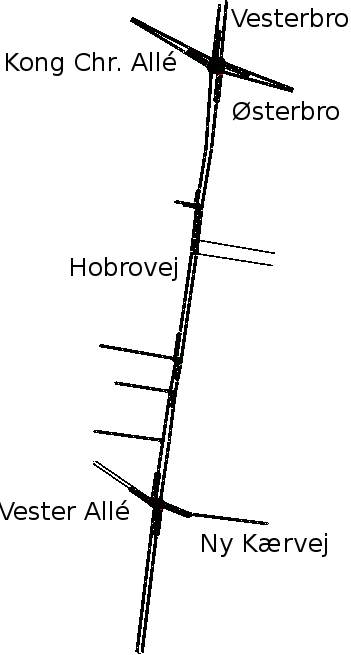
\includegraphics[width=0.15\textwidth]{images/Hobrovej.png}
\caption{Use case}
\label{fig:Introduction:hobro}
\end{figure}

Hobrovej has seven cross sections, of which two have complicated light signals, two has simpel light signals, and three does not have any light signals. %TODO: too inconcrete
The network is an exact replica of Hobrovej, with the same distance between sections, the same number of lanes and connections, the same traffic light signals.
The routes and the number of the vehicles on the network is also based on real observations from Hobro.
We only model vehicles of the types detailed in Tabel~\ref{tabel:vehicleTypes}, and do not model neither pedestrians nor cyclists.

%TODO: Explain routes
\begin{tabular}{|l|l|}\hline
\textbf{ID} & \textbf{Route}\\\hline
51 & Nord - syd\\\hline
\end{tabular}